\section{Stochastic Hill Climbing}

\subsection{Orientações}

Foi requerida uma implementação do Stochastic Hill Climbing, onde fossem observados e descritos os seguintes critérios:

\begin{itemize}
	\item Descrição da função objetivo utilizada na modelagem do problema
	\item Descrição da codificação utilizada para a solução candidata
	\item Descrição da(s) heurística(s) e o(s) critérios de parada utilizados pelo algoritmo.
	\item Execute 50 vezes o algoritmo e calcule: média e desvio padrão do número mínimo de	iterações necessário para parar o algoritmo; média e desvio padrão do tempo de	execução do algoritmo.
	\item Construa dois gráficos:
		\begin{itemize}
			\item 1) plotar a curva com número mínimo de iterações de cada execução.
			\item 2) plotar a curva com o tempo de execução do algoritmo de cada execução.
		\end{itemize}
	\item Mostre, pelo menos, duas soluções distintas encontradas pelo algoritmo.
	\item Comente e mostre o código fonte do algoritmo desenvolvido.
\end{itemize}

\subsection{Implementação}

A implementação do algoritmo foi feita na linguagem Python, pela ampla diversidade de bibliotecas funções, módulos e métodos disponíveis que facilitaram a estrutura dos dados e a legibilidade das instruções. Foram utilizadas as seguintes bibliotecas para a execução do algoritmo.

\lstinputlisting[name=foo, firstnumber=last,firstline=1, lastline=6]{../src/hill-climbing.py}

\subsubsection{Codificação da solução candidata}

O tabuleiro de xadrez do problema das oito rainhas pode ser facilmente abstraído computacionalmente em um array ou lista bidimensional, onde as casas vazias podem ser representadas por um inteiro $0$ e as ocupadas por rainhas representadas por um inteiro $1$. Entretanto tal representação armazena muitos dados que não interessam ao algoritmo, onde apenas as posições ocupadas pelas rainhas interessam. Tais representações esparsas devem ser evitadas, a fim de reduzir a complexidade computacional do algoritmo.

Com isso em mente, optou-se por usar uma representação mais condensada do tabuleiro. Uma lista de 8 posições, onde cada índice representa uma coluna, armazena um número que representa a linha, onde esses pares de valores de colunas e linhas são referências para as posições onde as oito rainhas estão. Note que isso também elimina a possibilidade de haver duas rainhas na mesma coluna, melhorando a solução do problema já na geração do mesmo. Dessa forma é possível mapear de maneira muito mais econômica as posições das rainhas.

A função \verb*|generate_random_solution()| retorna uma lista com oito listas internas, onde cada lista interna armazena 8 números inteiros gerados aleatoriamente sob uma distribuição uniforme de 0 a 7.

\lstinputlisting[name=foo, firstnumber=last,firstline=7, lastline=11]{../src/hill-climbing.py}

\subsubsection{Função Objetivo}

Como o objetivo do problema é fazer com que nenhuma rainha se ataque, a função de custo deve tender a diminuir, até um valor ótimo de 0 rainhas atacantes. Assim, a função objetivo foi projetada para que o problema seja de minimização, onde o valor de fitness do algoritmo indica a quantidade de rainhas que estão se atacando.

Duas rainhas estão se atacando quando elas estão presentes na mesma coluna, linha ou diagonal (em qualquer direção). A geração das soluções já eliminou a possibilidade de existirem rainhas na mesma coluna. Dessa forma, a função \verb*|calculate_fitness()| conta a quantidade de "colisões" para cada rainha do tabuleiro para a mesma linha (\verb*|[22]|) e para as quatro diagonais (\verb*|[25,30,35,40]|) e divide o total dessas colisões por 2, obtendo assim a quantidade de pares de rainhas atacantes.\\

\lstinputlisting[name=foo, firstnumber=last,firstline=12, lastline=46]{../src/hill-climbing.py}

\subsubsection{Heurísticas e Critérios de parada}

De posse das funções \verb*|generate_random_solution()| e \verb*|calculate_fitness()|, o corpo principal do algoritmo Stochastic Hill Climbing pode ser projetado.

Uma variável \verb*|max_cln| (\textit{maximum consecutive lateral movements}) indica o número máximo de movimentos laterais consecutivos do algoritmo, funcionando como um critério de parada caso o algoritmo fique preso num mínimo local. Como essa variável deve ser resetada caso o algoritmo saia do mínimo local, esse valor máximo permanece guardado, e \verb*|cln| é usado no decorrer do algoritmo. Durante a execução do algoritmo, optou-se por usar \verb*|cln| $=1000$.

Após inicializar uma solução aleatória e calcular sua respectiva fitness [54:55], um laço é iterado \verb*|58:72| até uma de duas condições de parada sejam atendidas:
\begin{itemize}
	\item Um valor de fitness seja 0, ou seja, onde é alcançado um estado em que nenhuma rainha se ataque.
	\item O algoritmo esgote sua cota de passos laterais e não encontre uma solução melhor.
\end{itemize}

Dentro do laço são geradas novas soluções que tem sua fitness comparada com a melhor obtida até então. Se uma solução superar a fitness da melhor solução, ela se torna a melhor. A função retorna uma lista contendo a melhor solução, seu valor de fitness e a quantidade necessária de iterações do laço até que um critério de parada fosse atendido. 

\lstinputlisting[name=foo, firstnumber=last,firstline=47, lastline=76]{../src/hill-climbing.py}

\subsection{Execução e Análise de resultados}

\subsubsection{Execução}

A fim de armazenar alguns dados das 50 execuções pedidas, foram criadas quatro listas \verb*|79:82|:
\begin{itemize}
	\item \verb*|solutions|: armazena as soluções das 50 execuções
	\item \verb*|fitnesses|: armazena os valores de fitness das 50 soluções
	\item \verb*|iterations|: armazena o número de iterações necessárias para as 50 execuções
	\item \verb*|runtimes|: armazena o tempo de execução de cada uma das 50 execuções. O cálculo do tempo foi feito através da diferença entre o tempo da CPU antes e depois da execução do Hill Climbing.
\end{itemize}

\lstinputlisting[name=foo, firstnumber=last,firstline=77, lastline=94]{../src/hill-climbing.py}

Foram obtidas as médias e desvios padrão das 50 iterações e tempos de execução.

\lstinputlisting[name=foo, firstnumber=last,firstline=95, lastline=109]{../src/hill-climbing.py}

Executando essas instruções, foram obtidos os seguintes dados:

\begin{figure}[H]
	\centering
	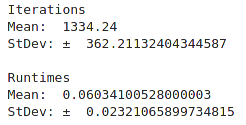
\includegraphics[scale=.7]{img/stats_hill}
	\caption{Média e desvio padrão de iterações e runtimes de 50 execuções}
	\label{statshill}
\end{figure}

\subsubsection{Gráficos}

O gráfico das iterações ao longo das execuções foi obtido usando a lista \verb*|iterations|:

\lstinputlisting[name=foo, firstnumber=last,firstline=110, lastline=120]{../src/hill-climbing.py}

Para os mesmos dados usados na figura (\ref{statshill}), foi obtida a seguinte plotagem:

\begin{figure}[H]
	\centering
	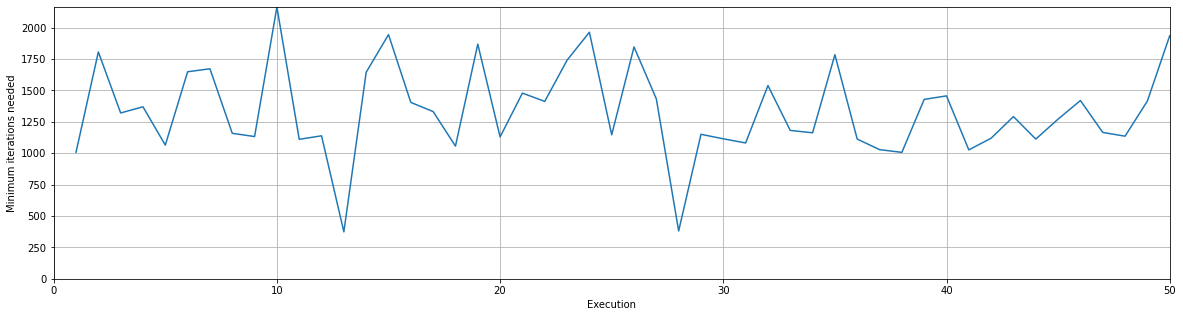
\includegraphics[width=\linewidth]{img/graph_1}
	\caption{Iterações ao longo das 50 execuções}
	\label{hill_iter}
\end{figure}

O gráfico dos tempos de execução ao longo das execuções foi obtido usando a lista \verb*|runtimes|:

\lstinputlisting[name=foo, firstnumber=last,firstline=121, lastline=131]{../src/hill-climbing.py}

Para os mesmos dados usados na figura (\ref{statshill}), foi obtida a seguinte plotagem:

\begin{figure}[H]
	\centering
	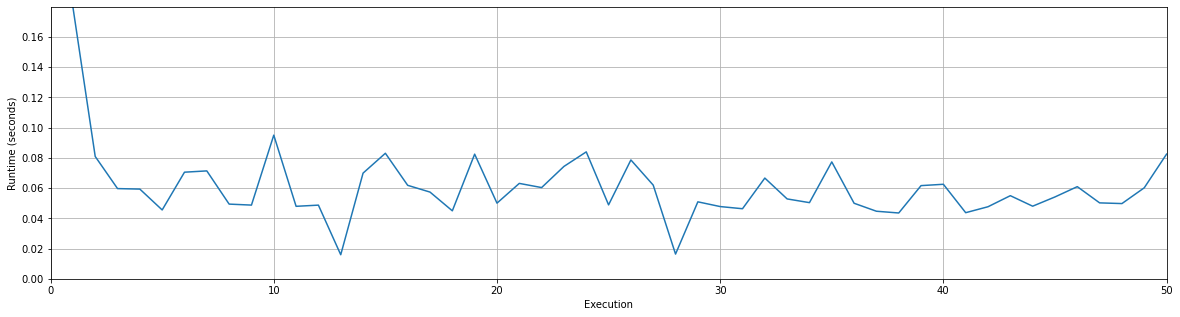
\includegraphics[width=\linewidth]{img/graph_2}
	\caption{Tempos de execução ao longo das 50 execuções}
	\label{hill_run}
\end{figure}

Podemos notar uma equivalência nas curvas dos dois gráficos, indicando uma relação direta ente a quantidade de iterações e o tempo de execução.

\subsubsection{Melhores soluções encontradas}

As 5 melhores soluções obtidas para a mesma execução da figura (\ref{statshill}) foram separadas e exibidas.

\lstinputlisting[name=foo, firstnumber=last,firstline=132, lastline=147]{../src/hill-climbing.py}

\begin{verbatim}
	Solution:  [4, 2, 0, 6, 1, 7, 5, 3]
	Fitness:  0
	----------------------------------
	Solution:  [5, 2, 0, 6, 4, 7, 1, 3]
	Fitness:  0
	----------------------------------
	Solution:  [0, 2, 5, 7, 4, 1, 3, 6]
	Fitness:  1
	----------------------------------
	Solution:  [1, 5, 4, 6, 3, 0, 2, 7]
	Fitness:  1
	----------------------------------
	Solution:  [2, 4, 6, 1, 3, 6, 0, 7]
	Fitness:  1
\end{verbatim}